\chapter{Entwicklung eines technischen Objekts}
%TODO Einleitung: Idee
% explizite Bezug auf Ultimaker 2, andere Drucker liefern andere Ergebnisse

Dieses Kapitel handelt vom Entwerfen und Drucken eines technischen Objekts. Als Objekt wird hier exemplarisch ein Aufbewahrungssystem f�r einen Raspberry Pi gekoppelt mit einem \ac{USB}- Hub und einer  externen Festplatte entworfen. Dieses System soll m�glichst kompakt sein und als ein Block transportierbar sein.

Diese Arbeit bezieht sich h�ufig auf den ultimaker 2, der im vorhergehenden Kapitel \ref{chapter:techGr:ultimaker2} vorgestellt wird. In der Arbeit mit einem anderen Drucker k�nnen sich Vorgehensweise und Ergebnis deutlich unterscheiden.

Zuerst wird die Analyse der bestehenden Verwahrung beschrieben. Anschlie�end folgt eine Beschreibung des umzusetzenden Konzepts. Folgend wird ein Entwurf des Systems mit einem \ac{CAD}-Programm  und der Druck des Objekts beschrieben. Der darauffolgende Abschnitt besch�ftigt sich mit w�hrend dem Druck aufgetretenen Fehlern. Zuletzt folgt ein Fazit �ber die Eignung des ultimaker 2 zum Drucken von technischen Objekten.


%TODO Ist-Analyse
\newpage
\section{Ist-Analyse}
	Zu entwerfen ist eine Verwahrung f�r einen Heimserver auf einem Raspberry Pi( folgend als Pi bezeichnet) mit angeschlossener externer Festplatte. Der Pi selbst liefert an seinen \ac{USB}-Ports nicht genug Leistung zum Betreiben der Festplatte, weshalb ein zus�tzlicher powered \ac{USB}-Hub n�tig ist. 
	
	\piccaption{Urspr�ngliches Stapelsystem\label{grafik:techObj:ursprStapelsystem}}
	\parpic{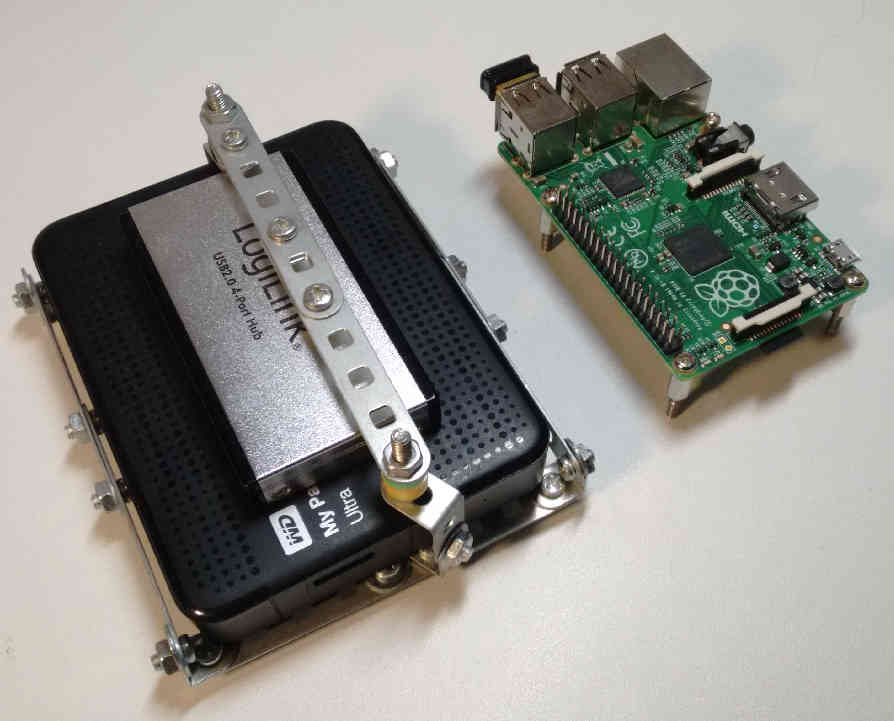
\includegraphics[width=.5\textwidth]{images/techObj/urspruenglicheHalterung02.jpg}}
	
	Zu Beginn der Entwicklung wurde das System durch zu einem K�fig verschraubten Lochblechen zusammengehalten, die Festplatte und Hub umfassten. Abbildung \ref{grafik:techObj:ursprStapelsystem} Insbesondere der Pi war im alten System nur unzureichend fixiert, da er nur auf den K�fig aufgesetzt war. Ein Hauptmerkmal des neuen Systems soll das sichere Lagern aller Komponenten sein. 
	
	\picskip{0}
	\vspace*{3em}
	
	N�chste Anforderung ist die Portabilit�t des Systems. Um den Server sicher und einfach bewegen zu k�nnen, soll das System als ganzes stabil zu einer Einheit verbindbar sein. Das bisherige System sollte die Portabilit�t erm�glichen, war jedoch aufgrund der oben genannten Instabilit�t nicht dazu in der Lage.  
	
	Die Ausma�e der zu verstauenden Objekte ist folgend aufgef�hrt.
	
	%TODO Messung Dimensionen
%	\begin{tabular}{c|c|c|c}
%		\label{}
%		\caption{�bersicht der Dimensionen der einzubauenden Objekte}
%				Bauteil 			& L�nge [mm] 	& Breite [mm]	& H�he [mm] \\ 
%		\hline 	Raspberry Pi 		& L�nge 	& Breite 	& H�he  \\ 
%				externe Festplatte 	& L�nge 	& Breite 	& H�he  \\ 
%				\ac{USB}-Hub 		& L�nge 	& Breite 	& H�he  \\ 
%		 
%	\end{tabular} 

	
	\begin{figure}
		
		
		\begin{minipage}[b]{.3\textwidth}
			
			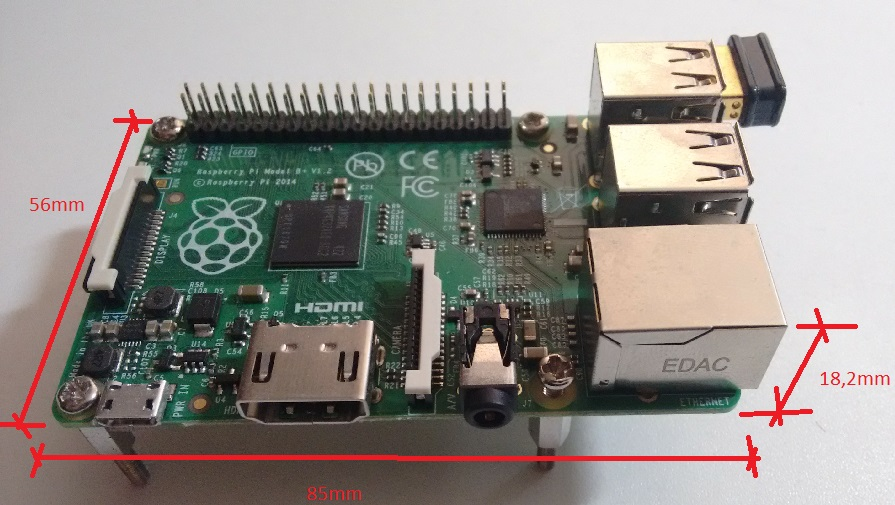
\includegraphics[width=\textwidth]{images/techObj/raspberry_bemasst}
			\subcaption{Bema�ung des Raspberry Pis}
			
		\end{minipage}
		\begin{minipage}[b]{.3\textwidth}
			
			
			\subcaption{Bema�ung des \ac{USB}-Hubs}
			
		\end{minipage}
		\begin{minipage}[b]{.3\textwidth}
			
			
			\subcaption{Bema�ung der externen Festplatte}
			
		\end{minipage}
		\label{Inhalt...}
		\caption{text}
	\end{figure}
	
	Zus�tzlich zu diesen Ma�en sind bei Pi noch die Positionen der Schraub-Bohrungen und die H�he der unter dem Pi herausragenden L�tpunkte und \ac{SMD}-Bauteile. Die frei zug�nglichen Leiterbahnen m�ssen in der Verwahrung Abstand zu anderen Bauteilen haben, da sie sonst besch�digt werden k�nnten.
	
	F�r das neue Verwahrungs-System soll eine Eigenschaft der alten �bernommen werden. Die Platzierung der Komponenten �bereinander ist sehr platzsparend und kann gut transportiert werden.

	
%TODO 
\section{Konzept: Modulare Boxen}

\section{Entwurf}
%Erw�hnen, dass Solid Edge verwendet

\section{Druck des Objekts}
% Wie w�re es ideal gewesen?, fertiges Objekt 
% Welche Parameter? --> spezifisch beim technischen Objekt
% Verlinkung zu Fehlern

\section{Aufgetretene Fehler}
% Bilder
% Fehleranalyse, [Ma�nahmen --> technische Grundlagen]

\section{Fazit: Eignung f�r technische Objekte}
% bezogen auf Ultimaker